% !TEX root = MSTAT19.tex
% This work is licensed under the Creative Commons
% Attribution-NonCommercial-ShareAlike 4.0 International License. To view a copy
% of this license, visit http://creativecommons.org/licenses/by-nc-sa/4.0/ or
% send a letter to Creative Commons, PO Box 1866, Mountain View, CA 94042, USA.

\section{Argmin-Theoreme in \texorpdfstring{$C(ℝ)$}{C(R)}} %8
Erinnere an folgende Probleme, vergleiche Gleichungen \eqref{eq1.2} und \eqref{eq1.5} in Kapitel \ref{sec:median} zum Median.
Wann überträgt sich die Konvergenz (f.\,s.\ oder in Verteilung) von stetigen stochastischen Prozessen auf deren Minimalstellen?

\begin{definition}\label{definition8.1}
	Sei $f∈ C(ℝ)$.
	\begin{enumerate}[label=(\arabic*)]
		\item $\begin{aligned}
			A(f):=\argmin(f):=\set{ t∈ℝ:f(t)=\inf_{s∈ℝ} f(s)}
			\end{aligned}$ = Menge aller Minimalstellen
		\item $τ∈ A(f)$ heißt \define{wohl-separiert}
			\begin{align*}
				:⇔\inf\set[\Big]{ f(t):\abs{t-τ}≥ε}>f(τ)\qquad∀ 0<ε∈ℚ
			\end{align*}
	\end{enumerate}
\end{definition}

\begin{bemerkungnr}\label{bemerkung8.2}\
	\begin{enumerate}[label=(\arabic*)]
		\item $A(f)\neq∅$ ist natürlich nicht ausgeschlossen, aber in jedem Fall ist $A(f)$ \emph{abgeschlossen} in $ℝ$, denn:
		Sei $(t_n)_{n ∈ ℕ}$ eine Folge in $A(f)$ mit $t_n \ntoinf t$. Dann gilt:
		\begin{align*}
			f(t)&=\limn\underbrace{f(t_n)}_{=\inf_{s∈ℝ}f(s)}=\inf_{s∈ℝ}f(s)
			⇒ t∈ A(f)
		\end{align*}
		\item $τ$ wohl-separiert $⇒τ$ eindeutig, denn:
		Sei $\tilde{τ}∈ A(f)$ und $\tilde{τ}\neqτ$. Also:
		\begin{align}\label{eqBemerkung8.2Stern}\tag{$\ast$}
			∃ 0 &< ε ∈ ℚ :
			\abs[\big]{τ - τ} > ε \\
			\nonumber
			\inf_{s∈ℝ}f(s)
			\overset{\tilde{τ}∈ A(f)}&=
			f(τ)
			\overset{\eqref{eqBemerkung8.2Stern}}{≥}
			\inf\set[\Big]{ f(t):\abs{t-τ}≥ε}
			\overset{τ\text{ wohl-sep}}{>}
			f(τ)
			\overset{τ∈ A(f)}{=}
			\inf_{s∈ℝ} f(s)
		\end{align}
		Dies ist ein Widerspruch!
		\item Wohl-separiertheit ist also eine stärkere Bedingung als Eindeutigkeit der Minimalstelle.
			Sie schließt \enquote{degenerierte} Fälle wie in Abbildung \ref{AbbMinimalstelleEindeutigNichtWohlsepariert} aus.
	\end{enumerate}
\end{bemerkungnr}

\begin{beisp}
	Wann ist eine Minimalstelle eindeutig, aber nicht wohlsepariert?
	\begin{figure}[H]
		\begin{center}
			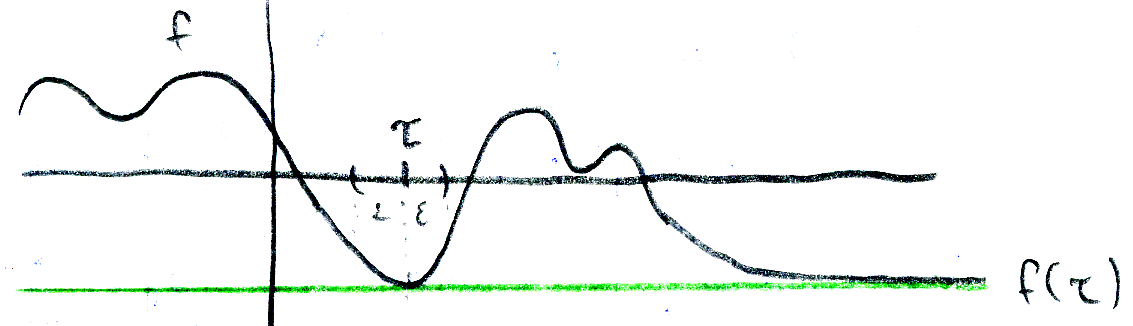
\includegraphics[width=1\textwidth]{./pics/MSTAT003.png}
			\caption{$τ$ eindeutig, aber das Infimum von $f$ außerhalb von $\intervallO{τ-ε}{τ+ε}$ ist auch $f(τ)$!}
			\label{AbbMinimalstelleEindeutigNichtWohlsepariert}
		\end{center}
	\end{figure}
\end{beisp}

\begin{satz}\label{satz8.3}
	Seien $f,f_n$, $n∈ℕ$ aus $C(ℝ)$, $τ_n∈ A(f_n)\neq∅~∀ n≥ N_0∈ℕ$
	(also $τ_n$ ist eine Minimalstelle, ab einem gewissen Zeitpunkt $N_0$.)
	und $τ∈ A(f)$ sei wohl-separiert.
	Falls
	\begin{align}\label{eqSatz8.3_1}\tag{1}
		\norm[\big]{ f_n-f}\overset{\text{Def}}{=}\sup_{t∈ℝ}\abs[\big]{f_n(t)-f(t)}\ntoinf 0
	\end{align}
	so folgt
	\begin{align*}
		τ_n\ntoinf τ
	\end{align*}
\end{satz}

\begin{proof}
	Sei o.\,B.\,d.\,A.\ $0 < ε ∈ ℚ$. Es folgt:
	\begin{align*}
		s(ε)&:=\inf\set[\big]{ f(t):\abs{t-τ}≥ε}
		\overset{\text{Def wohl-sep}}{>}
		f(τ)\\
		⇒
		δ &:= δ(ε) := \frac13 \klammern[\big]{s(ε) - f(τ)} > 0 \\
		\overset{\eqref{eqSatz8.3_1}}{⇒}
		∃ n_0&=n_0(δ)∈ℕ:∀ n≥ n_0:
		\norm{ f_n-f}≤δ
	\end{align*}
	Für alle $n≥\max(N_0,n_0)$ gilt:

	Falls $t∈ℝ$ mit $\abs{t-τ}≥ε$, so folgt:
	\begin{align*}
		f_n(t)-f_n(τ)
		&=\underbrace{f_n(t)-f(t)}_{≥\underbrace{-\underbrace{\norm{ f_n-f}}_{≤δ}}_{≥-δ}}+\underbrace{\underbrace{f(t)}_{≥ s(ε)}-f(τ)}_{≥ s(ε)-f(τ)=3δ}+\underbrace{f(τ)-f_n(τ)}_{≥-δ}\\
		&≥ -δ + 3δ - δ %\\
		%&
		= δ > 0
	\end{align*}
	Es folgt
	\begin{align}\label{eqProofSatz8.3Stern}\tag{$\ast$}
		f_n(t)>f_n(τ)\qquad∀ t∈ℝ\mit\abs{t-τ}≥ε
	\end{align}
	Folglich gilt $\abs{τ_n-τ}<ε$, denn sonst folgte aus \eqref{eqProofSatz8.3Stern}, dass
	$f_n(τ_n)>f_n(τ)$ im Widerspruch zu $τ_n$ ist Minimalstelle von $f_n$.

	Somit ist gezeigt:
	\begin{align*}
		∀ ε ∈ ℚ ∩ \intervallO0{∞} : ∃ m_0 = m_0(ε) := \max(N_0, n_0) : ∀ n ≥ m_0 : \abs{τ_n-τ} < ε
		& \qedhere
	\end{align*}
\end{proof}

Satz \ref{satz8.3} lässt sich problemlos von $ℝ$ auf offene Intervalle $I = \intervallO ab$ übertragen.

Für kompakte Intervalle $I=\intervall ab$, $a < b ∈ ℝ$ muss $τ$ nur eindeutig sein.
Es gilt:

\begin{satz}\label{satz8.4}
	Sei $I=\intervall ab$ kompaktes Intervall und seien $f,f_n$, $n∈ℕ$ aus $C(I)$.
	Dann gilt:
	\begin{enumerate}[label=(\arabic*)]
		\item \label{it:8.4argminexistenz} $\begin{aligned}
			A(f_n)\neq∅\qquad∀ n∈ℕ
		\end{aligned}$
		\item \label{it:8.4argminkonv} Falls $τ$ \emph{eindeutige} Minimalstelle von $f$ ist und falls
			\begin{align*}
				\norm{ f_n-f}_I:=\sup_{t∈ I}\abs[\big]{f_n(t)-f(t)}\ntoinf 0
			\end{align*}
			so gilt für \emph{jede} Auswahl $τ_n ∈ A(f_n)$:
			$τ_n\ntoinf τ$
	\end{enumerate}
\end{satz}

%Ferger: "In irgendeinem der Seminarräumen ist mal eine Tafel von der Wand gefallen. Und ich möchte jetzt nicht unter so einer Tafel begraben liegen.
% Vielleicht ist das für einen Professor ein schöner Tod. Aber bitte jetzt noch nicht."
% "Ich bin ja von Natur aus etwas ängstlich. Es gab da mal so ein lustiges Lied und da singt der Sänger: "Leute seid nicht feige, lasst mich ...""

\begin{proof}
	\ref{it:8.4argminexistenz} gilt, da jede stetige Funktion auf einem Kompaktum das Infimum annimmt.
	\paragraph{Zeige \ref{it:8.4argminkonv}:}
	$τ$ ist wohl-separiert auf $I$, denn:
	Angenommen, es wäre nicht so, also angenommen
	\begin{align*}
		∃0<ε∈ℚ:\inf\set[\big]{ f(t):t∈ I:\abs{t-τ}≥ε}=f(τ)
	\end{align*}
	Die Menge $K_ε:=\set{ t∈ I:\abs{t-τ}≥ε}$ ist kompakt.
	Weil $f$ stetig ist, nimmt $f$ auf $K_ε$ ihr Infimum an, d.\,h.
	\begin{align*}
		∃σ∈ I:\abs{σ-τ}≥ε\mit f(σ)=\inf
		\set[\big]{ f(t):t∈ I:\abs{t-τ}≥ε}
		=f(τ)
	\end{align*}
	Also ist $σ$ eine \emph{weitere} Minimalstelle von $f$ (denn $σ$ und $τ$ haben positiven Abstand zueinander) im Widerspruch zur Eindeutigkeit von $τ$.

	Jetzt weiter wie im Beweis von Satz \ref{satz8.3}.
\end{proof}

Es ergeben sich nun mühelos Argmin-Theoreme für fast sichere Konvergenz:

\begin{satz}\label{satz8.5}
	Seien $M=\set[\big]{ M(t):t∈ ℝ}$, $M_n=\set[\big]{ M_n(t):t∈ ℝ}$, $n∈ℕ$ stochastische Prozesse
	über $(Ω,\A,\P)$ mit Pfaden in $C(ℝ)$ (d.\,h.\ $M\colon ℝ⟶ℝ,~t↦ M(t,ω)$ stetig für alle $ω∈Ω$).
	Es gelte:
	\begin{enumerate}[label=(\arabic*)]
		\item \label{it:8.5tauIsMin} Es gilt
			\begin{align*}
				τ(ω)∈ A\klammern[\big]{M(·,ω)}\overset{\Def}{=}
				\argmin\klammern[\big]{M(·,ω)}
				\overset{\Def}{=} \set[\Big]{t ∈ R : \inf_{s ∈ ℝ} M(s, ω) = M(t, ω)}
				\text{f.\,s.}
			\end{align*}
			für eine Zufallsvariable $τ \colon Ω ⟶ ℝ$,
			also $\P\argu[\big]{\set[\big]{ω ∈ Ω : τ(ω) ∈ A\argu{M(·, ω)}}} = 1$
		\item \label{it:8.5wohlsep} $\begin{aligned}
			\inf \set[\big]{ M(t) : \abs{t - τ} ≥ ε} > M(τ) \text{ f.\,s. }\qquad ∀\, 0 < ε ∈ ℚ
		\end{aligned}$ (wohl-separiertheit)
		\item \label{it:8.5Konvergenz} $\begin{aligned}
			\norm[\big]{M_n-M}_∞\ntoinf 0\text{ f.\,s.}
		\end{aligned}$
	\end{enumerate}
	Dann gilt für jede Folge $(τ_n)_{n∈ℕ}$ von Zufallsvariablen mit $τ_n∈ A(M_n)$ f.\,s.:
	$τ_n\ntoinf τ$ f.\,s.
\end{satz}

\begin{proof}
	Setze
	\begin{align*}
		Ω_0 := \underbrace{
			\set[\Big]{ω ∈ Ω : τ(ω) ∈ A \argu[\big]{M(·, ω)}}
		}_{=: \set[\big]{τ ∈ A(M)} \text{ Einsmenge wg \ref{it:8.5tauIsMin}}}
		& ∩ \bigcap_{0 < ε ∈ ℚ}
		\overbrace{
			\underbrace{
				\set[\Big]{ \inf \set[\big]{ M(t) : \abs{t - τ} ≥ ε} > M(τ)}
			}_{\text{Einsmenge wg.\ \ref{it:8.5wohlsep}}}
		}^{ \hat{=} \text{wohl-separiert}}\\
		& ∩
		\underbrace{
			\set[\Big]{ \norm{ M_n - M} \ntoinf 0}
		}_{\text{Einsmenge wg \ref{it:8.5Konvergenz}}}
		∩ \bigcap_{n ≥ 1}
		\underbrace{
			\set[\Big]{τ_n ∈ A(M_n)}
		}_{\text{Einsmenge nach Vor.}}
	\end{align*}
	Erinnerung: Abzählbare Schnitte von Einsmengen sind Einsmengen.
	Dann gilt $\P(Ω_0)=1$.

	Satz \ref{satz8.3} besagt, dass für alle $ω ∈ Ω_0$ die Konvergenz
	der Mininmalstellen $τ_n(ω) → τ(ω)$ gilt. Also gilt $τ_n → τ$ fast sicher.
	% Da $Ω_0\overset{\ref{satz8.3}}{⊆}\set[\big]{τ_n\ntoinf τ}$, folgt die Behauptung.
\end{proof}

Analog erhält man mit Satz \ref{satz8.4}:

\begin{satz}\label{satz8.6}
	Seien $M,M_n,n∈ℕ$ stochastische Prozesse über $(Ω,\A,\P)$ mit Pfaden in $C(I)$,
	wobei $I$ kompaktes Intervall ist.
	Es gelte:
	\begin{enumerate}[label=(\arabic*)]
		\item \label{it:8.6eindeutig} Es gibt eine Zufallsvariable $τ$, die f.\,s.\ eindeutige Minimalstelle von $M$ ist.
		\item \label{it:8.6fskonvergenz} $\begin{aligned}
			\norm{ M_n-M}_I\ntoinf 0
		\end{aligned}$ f.\,s.
	\end{enumerate}
	Dann gilt für jede Folge $(τ_n)_{n∈ℕ}$ von Zufallsvariablen mit $τ_n∈ A(M_n)$ f.\,s.:
	$τ_n\ntoinf τ$ f.\,s.
\end{satz}

\begin{proof}
	Setze
	\begin{align*}
		 Ω_0&:=\set{τ\text{ ist eindeutige Minimalst. v. }M}
		 ∩\set[\Big]{\norm{ M_n-M}_I\ntoinf 0}
		 ∩\bigcap_{n≥1}\set[\Big]{τ_n∈ A(M_n)}\\
		 &⇒\P(Ω_0)=1
	\end{align*}
	Da $Ω_0\overset{\ref{satz8.4}}{⊆}\set[\Big]{τ_n\ntoinf τ}$, folgt die Behauptung.
\end{proof}


